\chapter{Performance Evaluation} \label{Performance Evaluation}
\section{Simulations Environment} \label{Simulations Environment}
A set of simulations were performed for evaluating the performance levels of existing Objective functions namely OF0 and mrhof. The simulations were performed under Contiki OS 2.6 which provides a network simulator called COOJA which permits the emulation of real hardware platforms. COOJA is the application of Contiki OS concentrating on network behavior. It is capable of simulating wireless sensor networks without any particular mote. Cooja supports the following set of standards; TR 1100, TI CC2420, Contiki-RPL, IEEE 802.15.4, uIPv6 stack and uIPv4 stack.\cite{3} There are 4 propagation models in COOJA simulator which must be selected for a simulation namely unit disk graph medium (UDGM): Distance loss, UDGM: Constant loss, Directed graph radio medium (DGRM), no radio traffic, multipath ray-tracer medium (MRM).\\
The simulations were conducted for 70, 90 and 100 motes using of0 and mrhof. All simulations were conducted using UDGM and same random seed for the same number of motes for Tmote sky motes.
\begin{figure}[h!]
\centering
\subfigure[random topology for 70 motes]
	{
	\label{fig:a}
	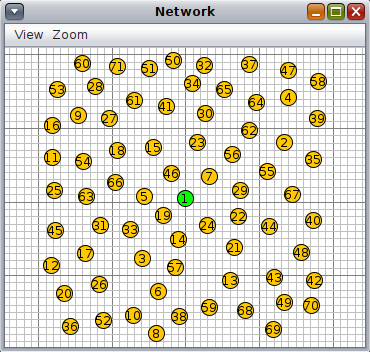
\includegraphics[width=50mm]{70.png}
	}
\subfigure[random topology for 90 motes]
	{
	\label{fig:b}
	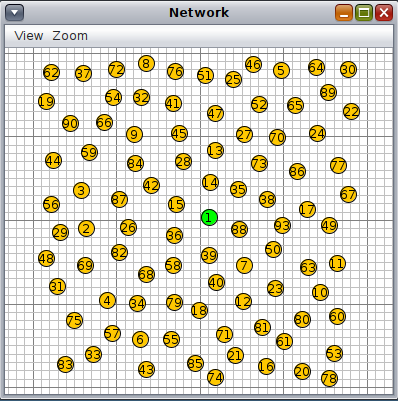
\includegraphics[width=50mm]{90.png}
	}
\subfigure[random topology for 100 motes]
	{
	\label{fig:b}
	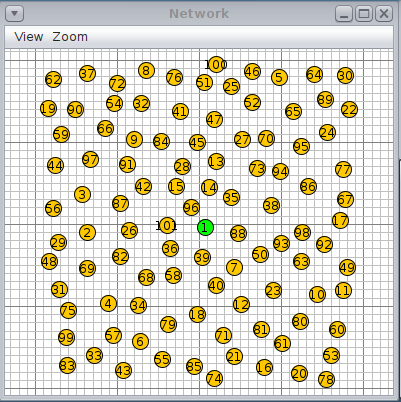
\includegraphics[width=50mm]{100.png}
	}
\caption{simulation of 70, 90 and 100 motes}
\label{fig:method}
\end{figure}
\noindent The performances of the two OFs were compared based on the following criteria:\\
\vspace{-1cm}
\begin{itemize}
\item Average latency: It refers to the average time a transmitted packet consumes from sender node to sink node. The following equation can be used for calculating it:\\
$ Average Latency = \frac{\Sigma_{k=1}^{n}recv\ time-send\ time}{total\ packets\ recieved} $
\item Packet delivery ratio (PDR): It refers to the ratio of nodes’ number of received and sent packets. The following equation can be used for calculating it:\\
$ Packet Delivery Ratio = \frac{total\ recieved\ packets} {total\ sent\ packets}  $
\item Energy consumption (mJ): Energy anode requires to exchanges data through the network between nodes. The following equation can be used for calculating it:\\
$ EnergyConsumption = \frac{(transmit*19.5mA\ +\ Listen*21.5mA\ +\ CPU_time*1.8mA + LPM*0.0454mA)*3V} {32768} $
\item Control traffic overhead: Represents the total number of control messages DIO, DAO \& DIS used by ICMPv6, it is calculated based on the following equation.\\
$ ControlTrafficOverhead = \Sigma_{1}^{n}DIO\ +\ \Sigma_{1}^{n}DIS\ +\ \Sigma_{1}^{n}DAO $
\end{itemize}

\subsection{Results of simulation} \label{Results of simulation}
The results obtained from the simulation were plotted using a python script to compare the two obejctive functions\\
\begin{figure}[H]
\centering
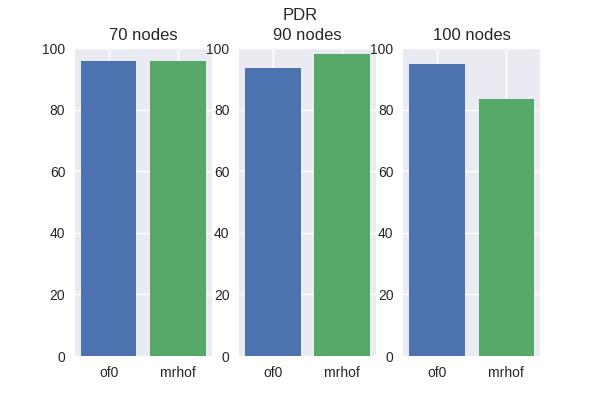
\includegraphics[width=70mm]{PDR.png}
\caption{Simulation plot for PDR}
\end{figure}
\textbf{PDR: }Power delivery ratio is seen to be almost equal for less dense network but is degraded to 83\% in case of Mrhof for a network of 100 nodes.\\
\begin{figure}[H]
\centering
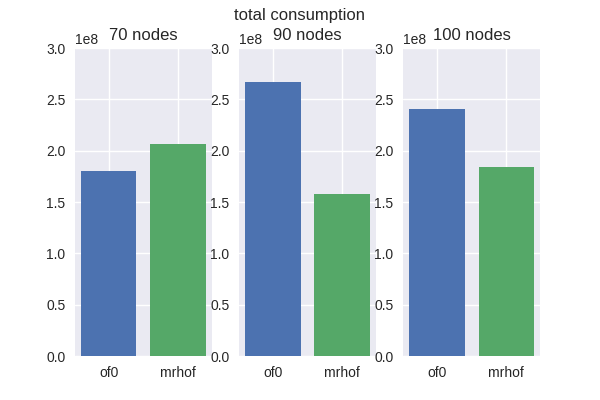
\includegraphics[width=70mm]{total consumption.png}
\caption{Simulation Plot for Energy}
\end{figure}
\textbf{ENERGY: }From this graph we can observe that mrhof performs better in terms of energy consumption for a large density of nodes
\begin{figure}[H]
\centering
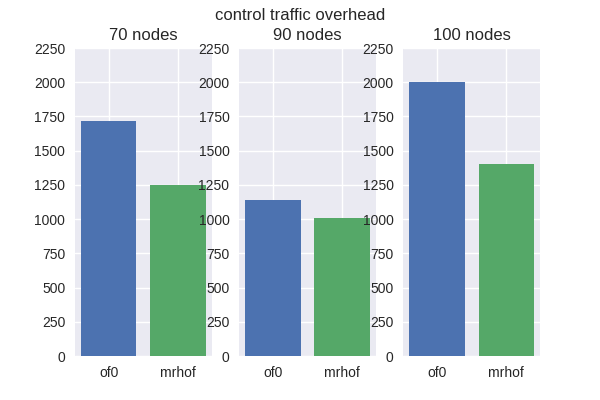
\includegraphics[width=70mm]{control traffic overhead.png}
\caption{Simulation Plot for Energy}
\end{figure}
\textbf{Control Traffic Overhead: }From this graph we can confirm that mrhof performs significantly better in terms of traffic overhead for large density networks
\begin{figure}[H]
\centering
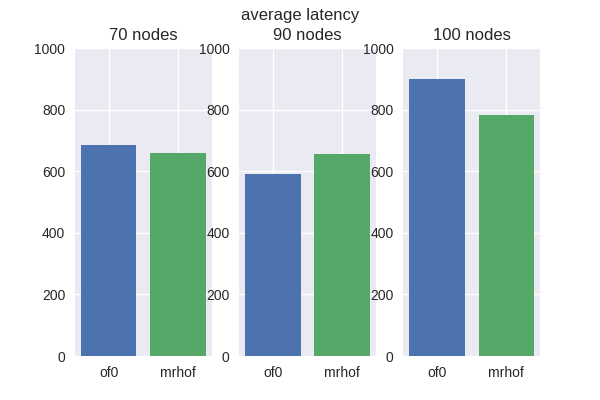
\includegraphics[width=70mm]{average latency.png}
\caption{Simulation Plot for Energy}
\end{figure}
\textbf{Average Latency: }Here we observe that mrhof has lower average latency as compared to OF0 for large networks
